\documentclass[letterpaper]{article}

\title{Problem Set 5}
\author{John L. Jones IV}
\date{MIT 6.0002 as Taught in Fall 2016 - \today}

\usepackage[utf8]{inputenc}
\usepackage[T1]{fontenc}
\usepackage{lmodern}
\usepackage{geometry} % Required for adjusting page dimensions and margins
\usepackage{graphicx}
\graphicspath{ {fig/} }


\begin{document}
	\maketitle
	\section*{Part A: Creating Models}
	\subsection*{Problem 4. Investigating the trend}
	\subsubsection*{Problem 4.I January 10th}
	\begin{figure}[h]
		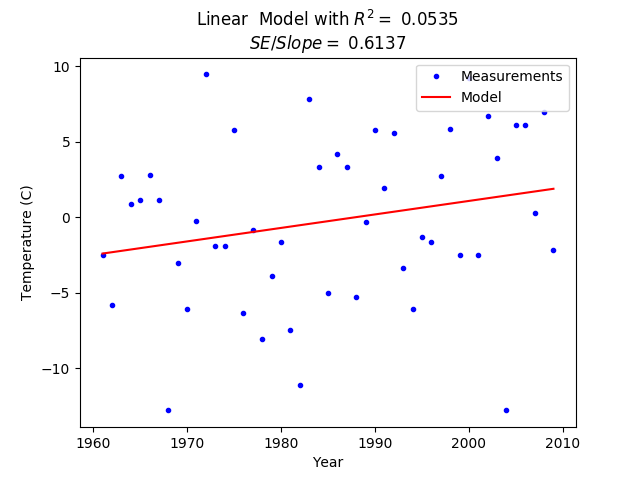
\includegraphics[scale=0.625]{Figure_1_A4I}
		\centering
		\caption{Temperature on January 10th in New York through training years.}
		\label{fig:Jan 10 NY}
	\end{figure}
	The best fitting linear model for a random day (January 10) resulted with $R^2 = 0.0535$ as shown in Figure \ref{fig:Jan 10 NY}.
	The $SE/slope$ for Figure \ref{fig:Jan 10 NY} is $0.6137$ for the purposes of this study $R^2 > 0.5$ indicates the trend is likely due to chance.
	When observing climate change, a yearly average should remove some of the "day-to-day" noise.
	Weather is more difficult to predict than climate.
	Daily weather changes introduce high frequency noise. Average with respect to time acts as a low-pass filter.
	\subsubsection*{Problem 4.II Annual Temperature}
	\begin{figure}[h]
		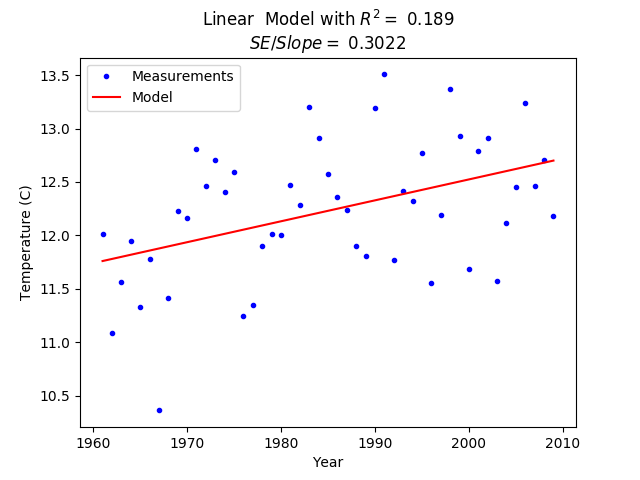
\includegraphics[scale=0.625]{Figure_2_A2II}
		\centering
		\caption{Annual average temperature in New York through training years.}
		\label{fig:Yearly Average NY}
	\end{figure}
	
	The same model-generating algorithm was used on the yearly average data and produced a best fitting line with an $R^2 = 0.189$ as shown in Figure \ref{fig:Yearly Average NY}.
	The $SE/slope$ for Figure \ref{fig:Yearly Average NY} is $0.3022$ indicating the trend may not be due to chance.
	There is likely less variance due to noise in the yearly average data allowing a trend over time to be more apparent.
	Both Figure \ref{fig:Jan 10 NY} and \ref{fig:Yearly Average NY} indicate temperate increasing on the order of $\frac{1}{2}$ degrees Celsius per $50$ years.
	The annual temperature study more strongly supports this trend than the random day study.

	\section*{Part B: Incorporating More Data}
	\begin{figure}[h]
		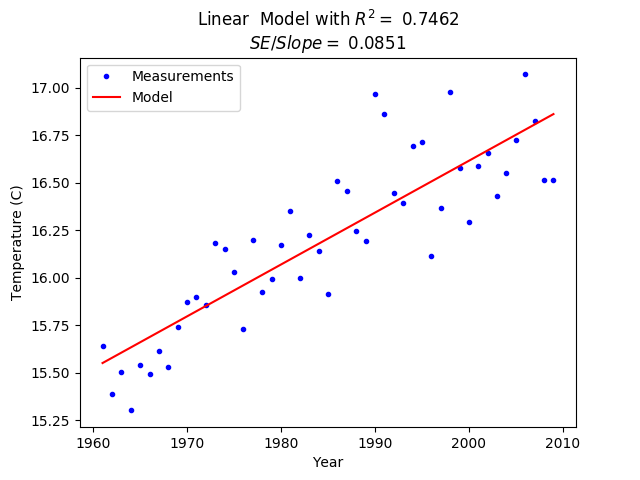
\includegraphics[scale=0.625]{Figure_3_B}
		\centering
		\caption{Yearly average across multiple cities.}
		\label{fig:Cities Avg}
	\end{figure}
	When including more cites a better picture of the global climate can be observed, especially cities that are geographically diverse.
	Much of the noise due to local weather variations can be averaged across multiple cities located in different regions.
	One would expect as more geographically independent cities are used in the model, the less power local weather noise has.
	There appears to be much less variance in this data compared to the single-city data previously analyzed.
	The $R^2 = 0.7462$ and $SE/Slope = 0.0851$ shown in Figure \ref{fig:Cities Avg} make a strong argument that this model for these cities indicating increasing yearly temperate is not likely to be due to chance or randomness.

	\section*{Part C: 5-year Moving Average}
	\begin{figure}[h]
		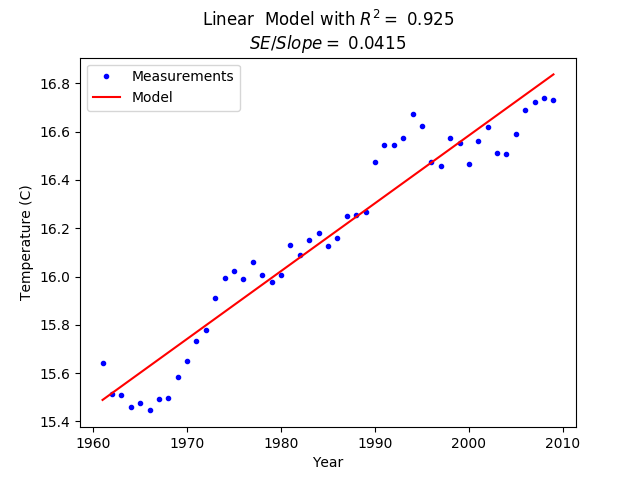
\includegraphics[scale=0.625]{Figure_4_C}
		\centering
		\caption{Yearly average across multiple cities using 5-year moving average filter.}
		\label{fig:Moving Avg}
	\end{figure}
	More high frequency noise can be removed with a moving average filter in addition to geographic averaging.
	We are only interested in the long term climate change so any loss of high frequency signals such as weather variations or an outliers is acceptable.
	The $R^2 = 0.925$ and $SE/Slope = 0.0415$ shown in Figure \ref{fig:Moving Avg} make a strong argument that this model for these cities indicating increasing yearly temperate is not likely to be due to chance or randomness.
	This stronger $R^2$ and $SE/Slope$ is likely the result of reducing variance in the training data with the moving average filter.

	\section*{Part D: Predicting the Future}
	\subsection*{Problem 2.I Generate More Models}
	\begin{figure}[h]
		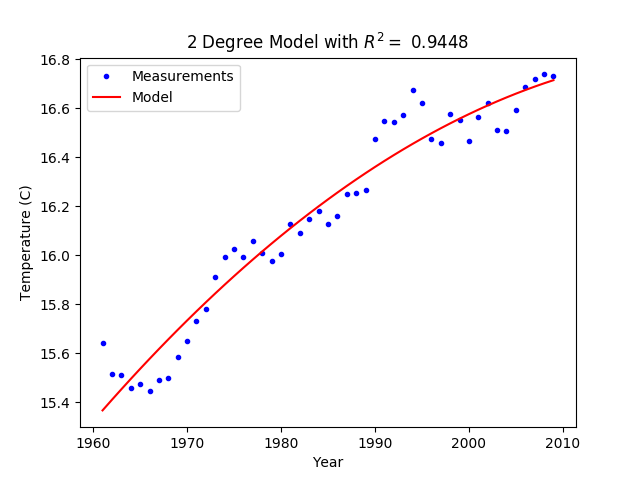
\includegraphics[scale=0.625]{Figure_5_D2I_2degree}
		\centering
		\caption{Training evaluation with 2-degree model.}
		\label{fig:2 degree training}
	\end{figure}\begin{figure}[h]
		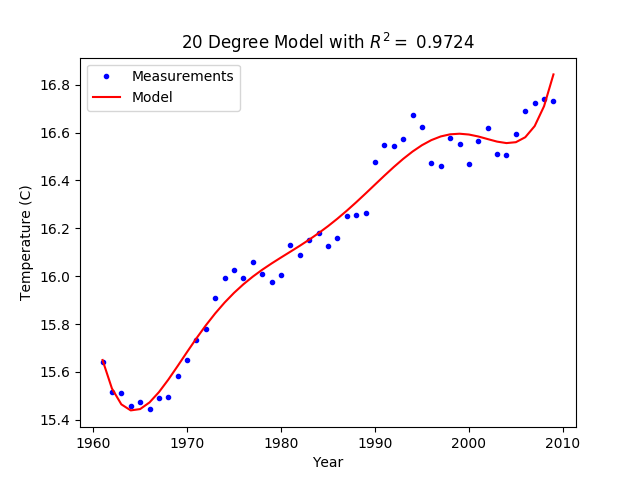
\includegraphics[scale=0.625]{Figure_6_D2I_20degree}
		\centering
		\caption{Training evaluation with 20-degree model.}
		\label{fig:20 degree training}
	\end{figure}
	The 20-degree model shown in Figure \ref{fig:20 degree training} has the lowest $R^2 = 0.9724$ value.
	A higher $R^2$ value indicates the model variance is small in comparison to the data variance i.e a better fit.
	However, the 20-degree model likely has been over-fit to the training data.
	It is very unlikely the underlying system of climate has any $x^{20}$ terms.
	Although the 20-degree model closely fits the training data, new climate data may not be accurately predicted with this high-order model.
	The linear and quadratic models shown in Figures \ref{fig:Moving Avg} and \ref{fig:2 degree training} seem to be the simplest and best solutions for predicting future values, despite the slightly lower values of $R^2 = 0.925$ and $R^2 = 0.9448$ respectively.

	\subsection*{Problem 2.II Predict the Results}
	\begin{figure}[h]
		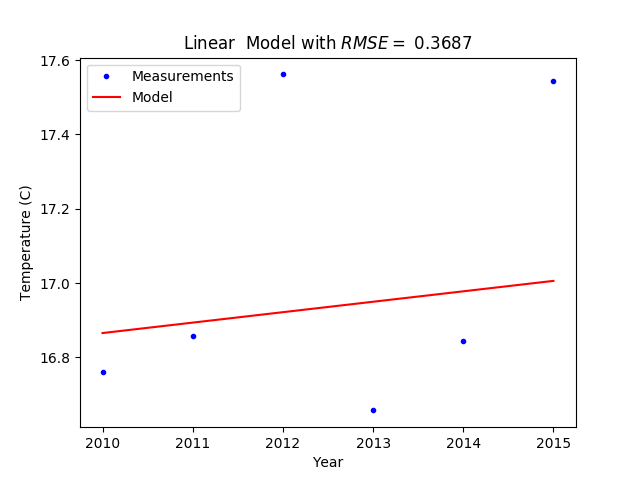
\includegraphics[scale=0.625]{Figure_7_D2II_linear}
		\centering
		\caption{Testing evaluation with linear model.}
		\label{fig:Linear testing}
	\end{figure}
	\begin{figure}[h]
		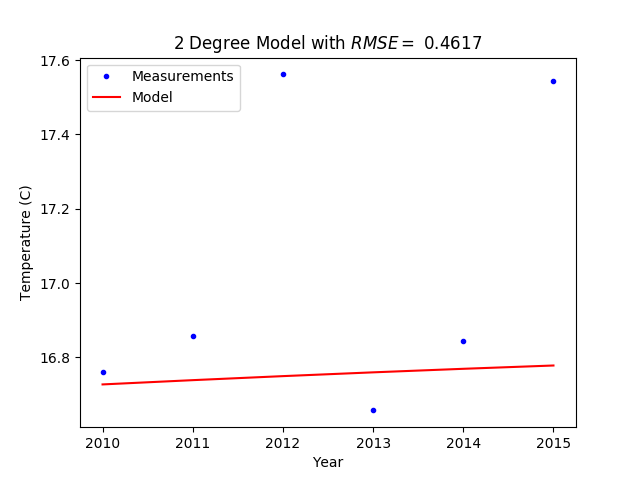
\includegraphics[scale=0.625]{Figure_8_D2II_2degree}
		\centering
		\caption{Testing evaluation with 2-degree model.}
		\label{fig:2 degree testing}
	\end{figure}\begin{figure}[h]
		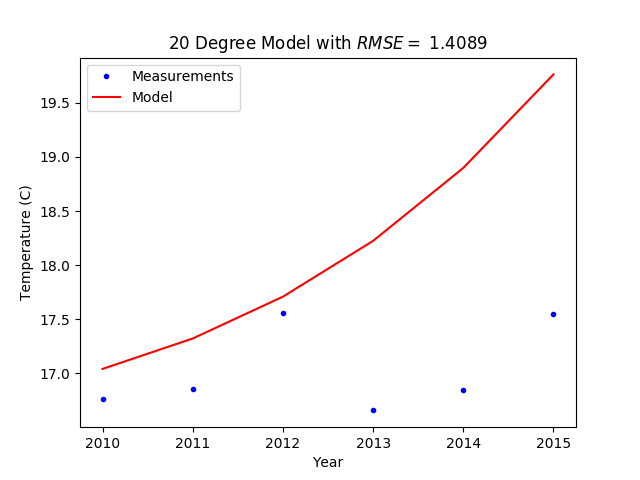
\includegraphics[scale=0.625]{Figure_9_D2II_20degree}
		\centering
		\caption{Testing evaluation with 20-degree model.}
		\label{fig:20 degree testing}
	\end{figure}
	When tested against future data, the linear model results in the lowest Root-Mean-Squared Error $RMSE = 0.3687$.
	The 2-degree model also performs well with $RMSE = 0.4617$. 
	The 20-degree model quickly diverges away from the future data as seen in Figure \ref{fig:20 degree testing}.
	When evaluated using future data, the linear model appears to be the best predictor of climate change over time.
	As demonstrated here, a model that is the best fit for a set of training data, does not always perform the best at predicting future data.
	If the models were trained using only the unfiltered temperatures of New York, there would likely be a "DC" bias since NYC seems to have a lower average temperature than world average temperature.
	\begin{figure}[h]
		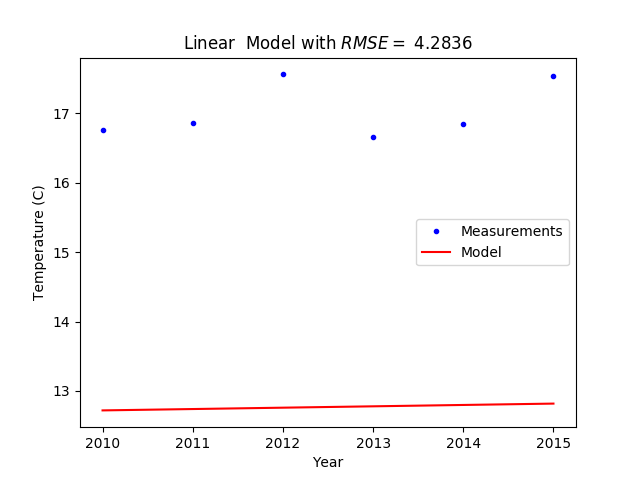
\includegraphics[scale=0.625]{Figure_10_NYC_vs_world}
		\centering
		\caption{NYC annual average model tested against world average temperatures.}
		\label{fig:NYC vs world}
	\end{figure}
	\begin{figure}[h]
		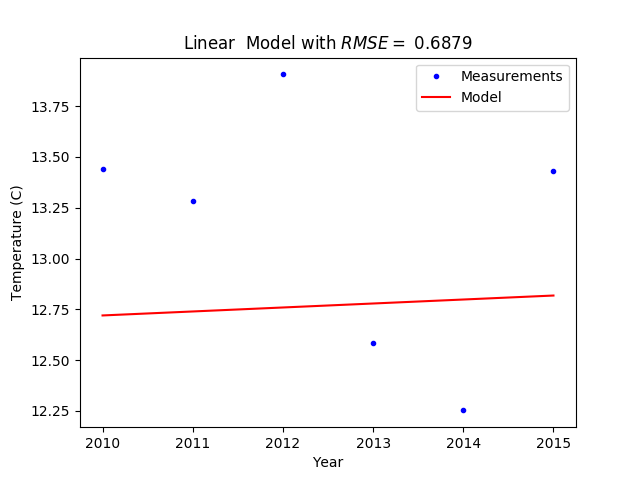
\includegraphics[scale=0.625]{Figure_11_NYC_vs_future_NYC}
		\centering
		\caption{NYC annual average model tested against NYC average temperatures.}
		\label{fig:NYC vs future NYC}
	\end{figure}
	Out of curiosity, I plotting the result in Figure \ref{fig:NYC vs world}.
	This same linear model from average New York data does a better job predicting temperatures in New York, see Figure \ref{fig:NYC vs future NYC}. 
	There is still a much higher $RMSE$ than the models produced using many cities.
	
	\section*{Part E: Modeling Extreme Temperatures}
	\begin{figure}[h]
		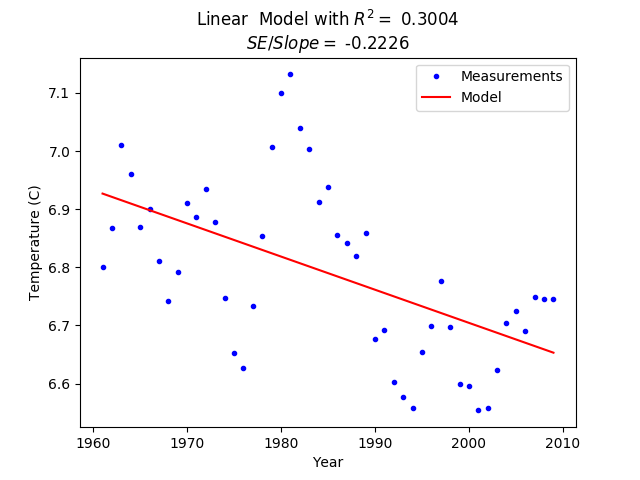
\includegraphics[scale=0.625]{Figure_12_std}
		\centering
		\caption{Model trained on temperature standard deviation over multiple cities.}
		\label{fig:std}
	\end{figure}
	This result does not support the claim that temperatures are getting more extreme.
	The negative slope in Figure \ref{fig:std} indicates there is less variance in temperature as time progresses.
	It may be better to average the standard deviations of locations instead of taking the standard deviation of the averages.
	The average temperature of many cities to indicate may not indicate extreme changes within the individual cities.

\end{document}
